\documentclass[19pt,a4paper]{article}
\usepackage{xeCJK}
\usepackage{amsmath}
\setmainfont{STSong}
\usepackage{geometry}
\geometry{left=2.5cm,right=2.5cm,top=2.5cm,bottom=2.5cm}
\setlength{\parindent}{4em}
\usepackage{graphicx}
\usepackage{float}
\title{第二次实验报告}
\author{王诗俊2015201951\quad 廖钰蕾2015201953\quad  孟妍廷2015202009\quad  刘笑2015201925}
\date{2017年11月4日}

\begin{document}
\maketitle

\textbf{一\quad 目标:}\\
\indent 1.替换上一阶段损坏的电池\\
\indent 2.利用手机蓝牙控制小车行驶\\
\indent 3.在小车上固定开启着摄像头的手机,手机通过WiFi将摄像头所拍画面实时传至电脑端\\
\indent 4.电脑端每隔2s截一张图,根据自己训练出的模型选择合适的转弯方向\\
\indent 5.对图像进行处理,使小车能够识别红绿色,“红灯停,绿灯行”\\
\\
\\
\indent\textbf{二\quad 收集数据:}\\ 
\indent 1.数据要求\\
\indent\ \ 小车在实际行驶过程中以不同角度靠近墙壁的图片\\
 \\
\indent 2.数据获取\\
\indent\ \ (1)电脑端安装DroidCam软件,手机端(固定在小车上)安装对应APP,连在同一局域网\\
\indent\ \ (2)手机端打开摄像头,电脑端能看到手机拍摄的实时画面(WiFi状况良好的情况下)\\
\indent\ \ (3)电脑端安装Python的opencv包,编写py程序调用此包,程序功能是每隔2s截一张图片并\\
\indent \ 保存\\
\indent\ \ (4)人为控制:\\
\indent\ \ \ \ $\cdot$手动控制小车撞墙的角度,保证角度多样化\\
\indent\ \ \ \ $\cdot$在小车撞墙后,手动将小车与墙壁分离\\
\indent\ \ \ \ $\cdot$在小车翻车后,手动将小车扶正\\
\indent\ \ \ \ $\cdot$在小车零件被震翻、线路被震断时,手动恢复\\
\\
\indent 3.时刻关注电脑端的截图、WiFi连接状况和截图完成情况\\
\\
\indent 4.数据筛选\\
\indent\ \ (1)剔除了各种“人类无法识别”的图片(WiFi刚连接的前几张图片为纯色的、WiFi连接不稳定\\
\indent\ \ 时的图片会错位)\\
\begin{figure}[H]
 \centering
 
\includegraphics[scale=0.4]{2.png}
\end{figure}
\begin{figure}[H]
 \centering
 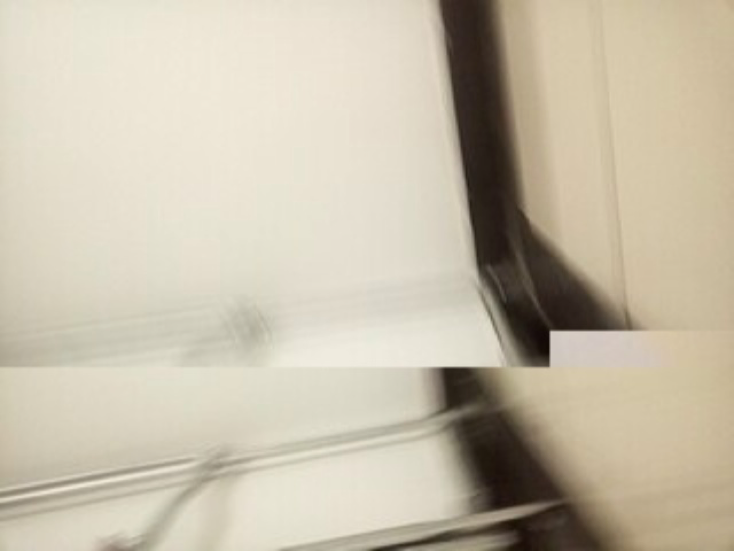
\includegraphics[scale=0.4]{1.png}
\end{figure}
\indent\ \ (2)剔除了各种“非撞墙”的图片(天花板、楼道里来来往往的人、地板上的小虫子、蹲在电脑前\\
\indent\ \ 监控拍摄进展的队友)\\
\begin{figure}[H]
 \centering
 
\includegraphics[scale=0.4]{3.png}
\end{figure}
\begin{figure}[H]
 \centering
 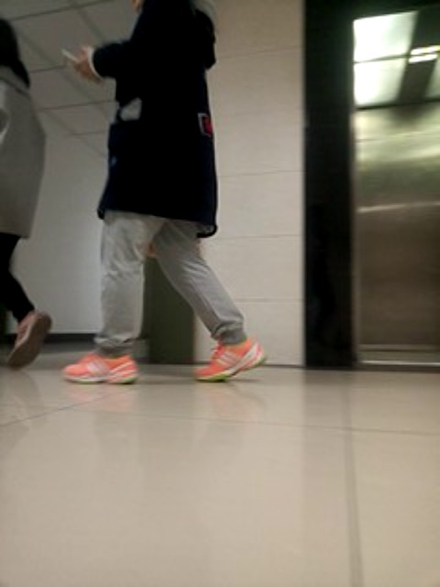
\includegraphics[scale=0.4]{4.png}
\end{figure}
\begin{figure}[H]
 \centering
 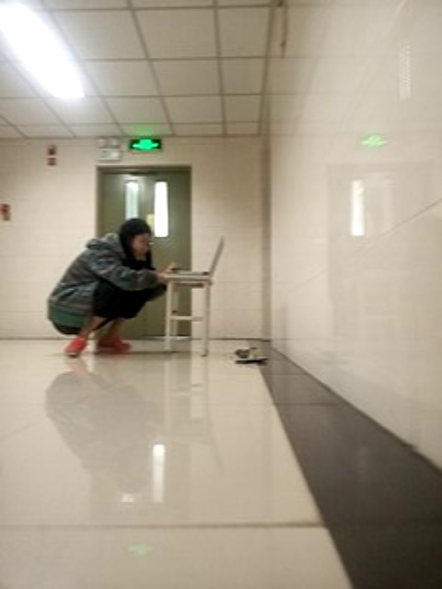
\includegraphics[scale=0.4]{5.png}
\end{figure}
\indent\ \ (3)剔除了各种“无法标注”的图片(离墙太远(无需转弯)、离墙太近(整个图片都是白花花/灰惨\\
\indent\ \ 惨/黑漆漆的墙壁))\\
\begin{figure}[H]
 \centering
 
\includegraphics[scale=0.4]{6.png}
\end{figure}
\begin{figure}[H]
 \centering
 
\includegraphics[scale=0.4]{7.png}
\end{figure}
\begin{figure}[H]
 \centering
 
\includegraphics[scale=0.4]{8.png}
\end{figure}
\indent 5.数据量\\
\indent\ \ 原始数据量:2600张图片(26个字母、每个字母100张)\\
\indent \ \ 筛选后数据量:1787张图片 \\
\\
\\
\indent\textbf{三\quad 代码逻辑:}\\
\indent ——训练模型\\
\indent 1.图片预处理\\
\indent \ \ 对图片灰度处理,使用高斯平滑处理图片降噪,再使用Canny边检测器检测物体边际\\
\\
\indent 2.特征提取\\
\indent \ \ 用SIFT(尺度不变特征变换)来提取特征点,得到nx128的特征向量(n为特征点个数)\\
\\
\indent 3.向量量化\\
\indent \ \ (1)利用词袋模型对向量进行聚类,将每一簇向量看成一个“词”,将一幅画看成一个“袋”。\\
\indent \ \ (2)利用k-means算法提取所有图片的SIFT特征,若共有n个向量,将这n个向量划分成k类,\\
\indent\ \ 对每一维SIFT特征,均映射到一维上。\\
\indent \ \ (3)计算每个图片中的每一类向量出现的频率,做归一化处理。\\
\\
\indent 4.模型调优\\
\indent\ \ 采取SVM模型,采用GridSearchCV函数在参数范围内自动调优,寻找最优超参数,范围如下:\\
\indent$parameter_grid = [\\	
\indent\quad	{‘kernel’: [‘linear’], ‘class_weight’: [‘balanced’], ‘gamma’: [0.01, 0.001], ‘C’: [0.5, 1, 10, 50]},\\	
\indent\quad	{‘kernel’: [‘poly’], ‘class_weight’: [‘balanced’], ‘gamma’: [0.01, 0.001], ‘degree’: [2, 3]},\\	
\indent\quad	{‘kernel’: [‘rbf’], ‘class_weight’: [‘balanced’], ‘gamma’: [0.01, 0.001], ‘C’: [0.5, 1, 10, 50]},\\
\indent]$\\
\indent\ \ 最优模型保存在“svm.model”中\\
\\
\indent ——运行过程\\
\indent 1.读取模型\\
\indent 2.实时截取图片,并做红绿判断---将RGB图像转化为HSV图像,遍历图像判断红绿色彩\\
\indent 3.发送信号获取传感器距离信息\\
\indent 4.离墙较近时,对图片进行预处理,特征提取,向量量化等,并使用SVM进行分类,决定转\\
\indent 弯方向,返回给小车\\
\\
\\
\indent\textbf{四\quad 遇到的问题:}\\
\indent 1..收集数据的效率较低,只能靠人工慢慢控制,数据量较少。\\
\indent 2.筛选数据时每位成员的标准不同,导致筛选效率不够高\\
\indent 3.由于OpenCV的版本不同,成员在检查代码的时候出现了目前不知道如何调试的错误\\
\\
\\
\indent\textbf{五\quad 成果:}\\
\indent 1.小车
\begin{figure}[H]
 \centering
 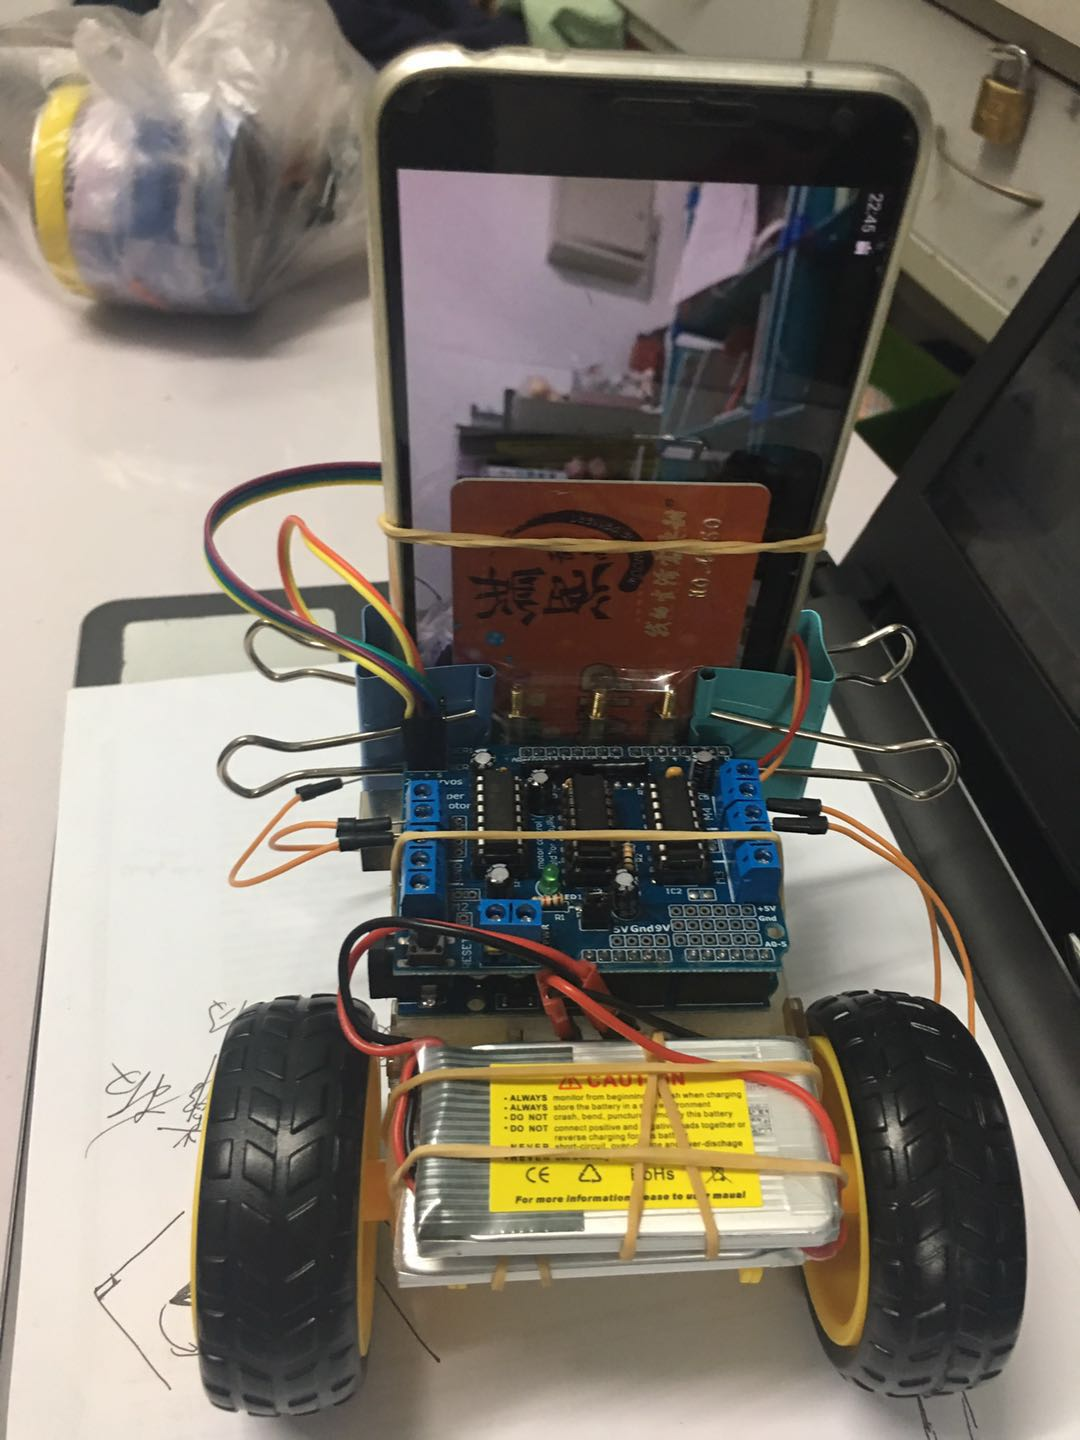
\includegraphics[scale=0.2]{2.jpeg}
\end{figure}
\indent 2.收集数据
\begin{figure}[H]
 \centering
 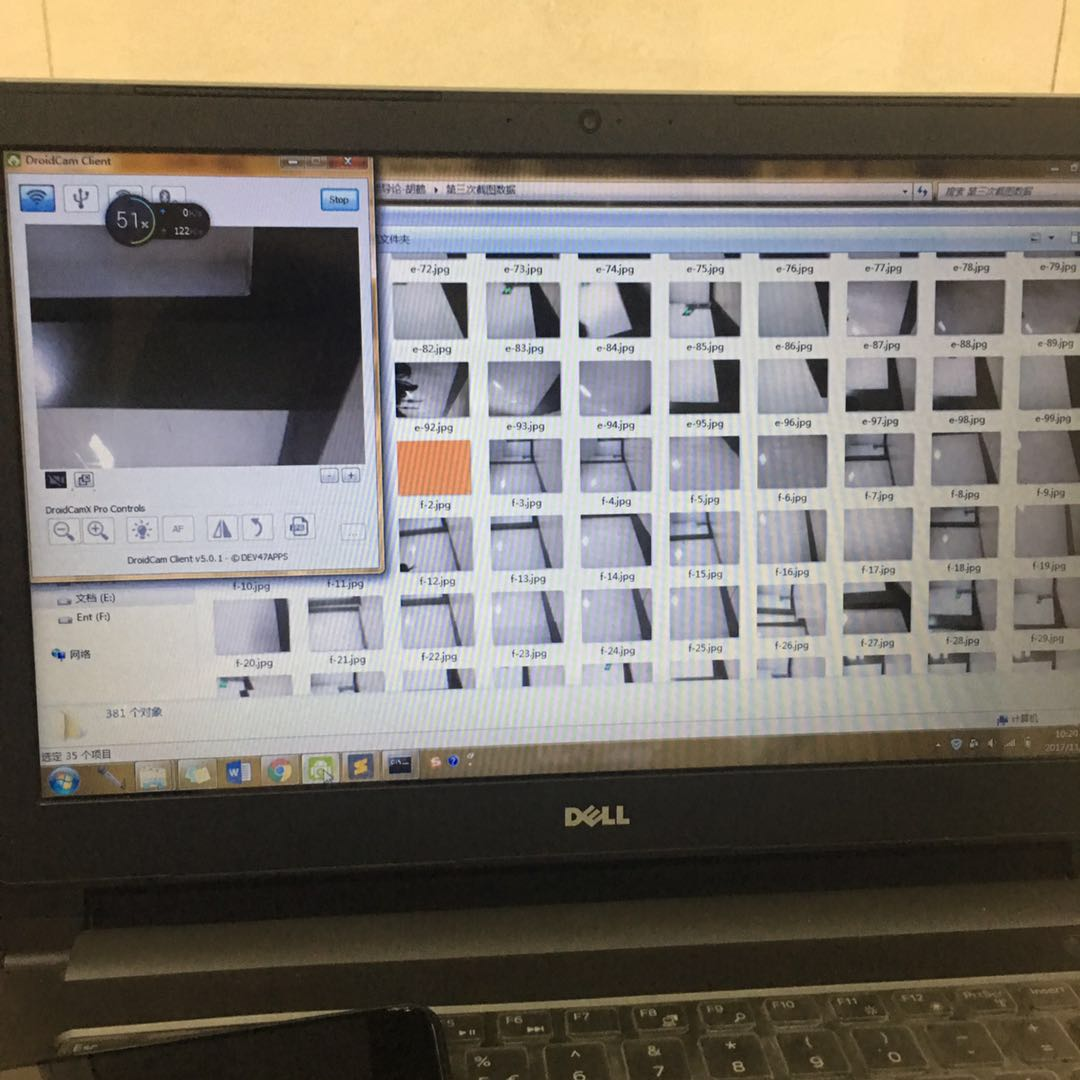
\includegraphics[scale=0.2]{4.jpeg}
\end{figure}
\indent 3.训练结果
\begin{figure}[H]
 \centering
 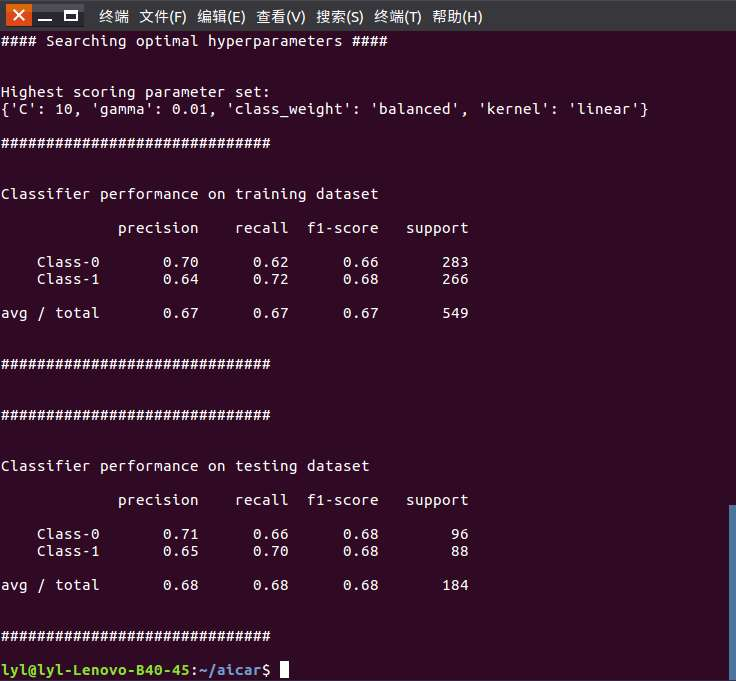
\includegraphics[scale=0.4]{5.jpeg}
\end{figure}
\indent 4.不同SVM得到的结果表
\begin{figure}[H]
 \centering
 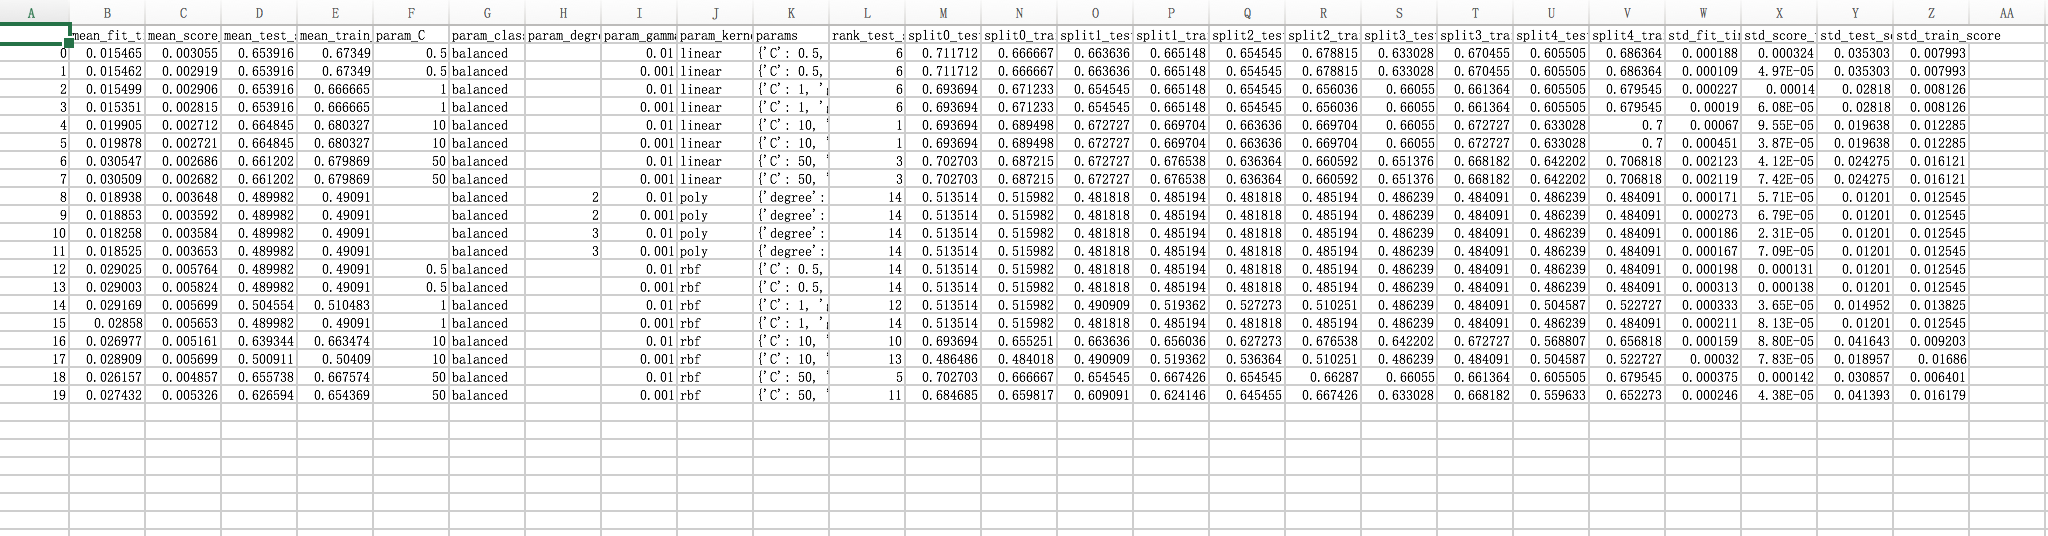
\includegraphics[scale=0.4]{6.jpeg}
\end{figure}
\indent 5.小车行驶见视频\\
\\
\\
\indent\textbf{六\quad 模型评价:}\\
\indent 1.图片预处理:用Canny处理过的图片能明显看到物体边,且降噪效果相对拉普拉斯等边检\\
\indent 测器好\\
\indent 2.每个图片的特征点个数不同,而SIFT是CV中常用的特征之一\\
\indent 3.向量量化:在计算机视觉中,SIFT向量维度较高,运算速度慢,可以在此对向量进行聚\\
\indent 类,而词袋模型最初用于文本分析领域,将每个文档看成袋子,根据袋中词语进行分类。\\
\indent 又由于每幅图对应多个向量,且个数不定,所以需要做归一化处理。\\
\\
\\
\indent\textbf{七\quad 分工:}\\
\begin{figure}[H]
 \centering
 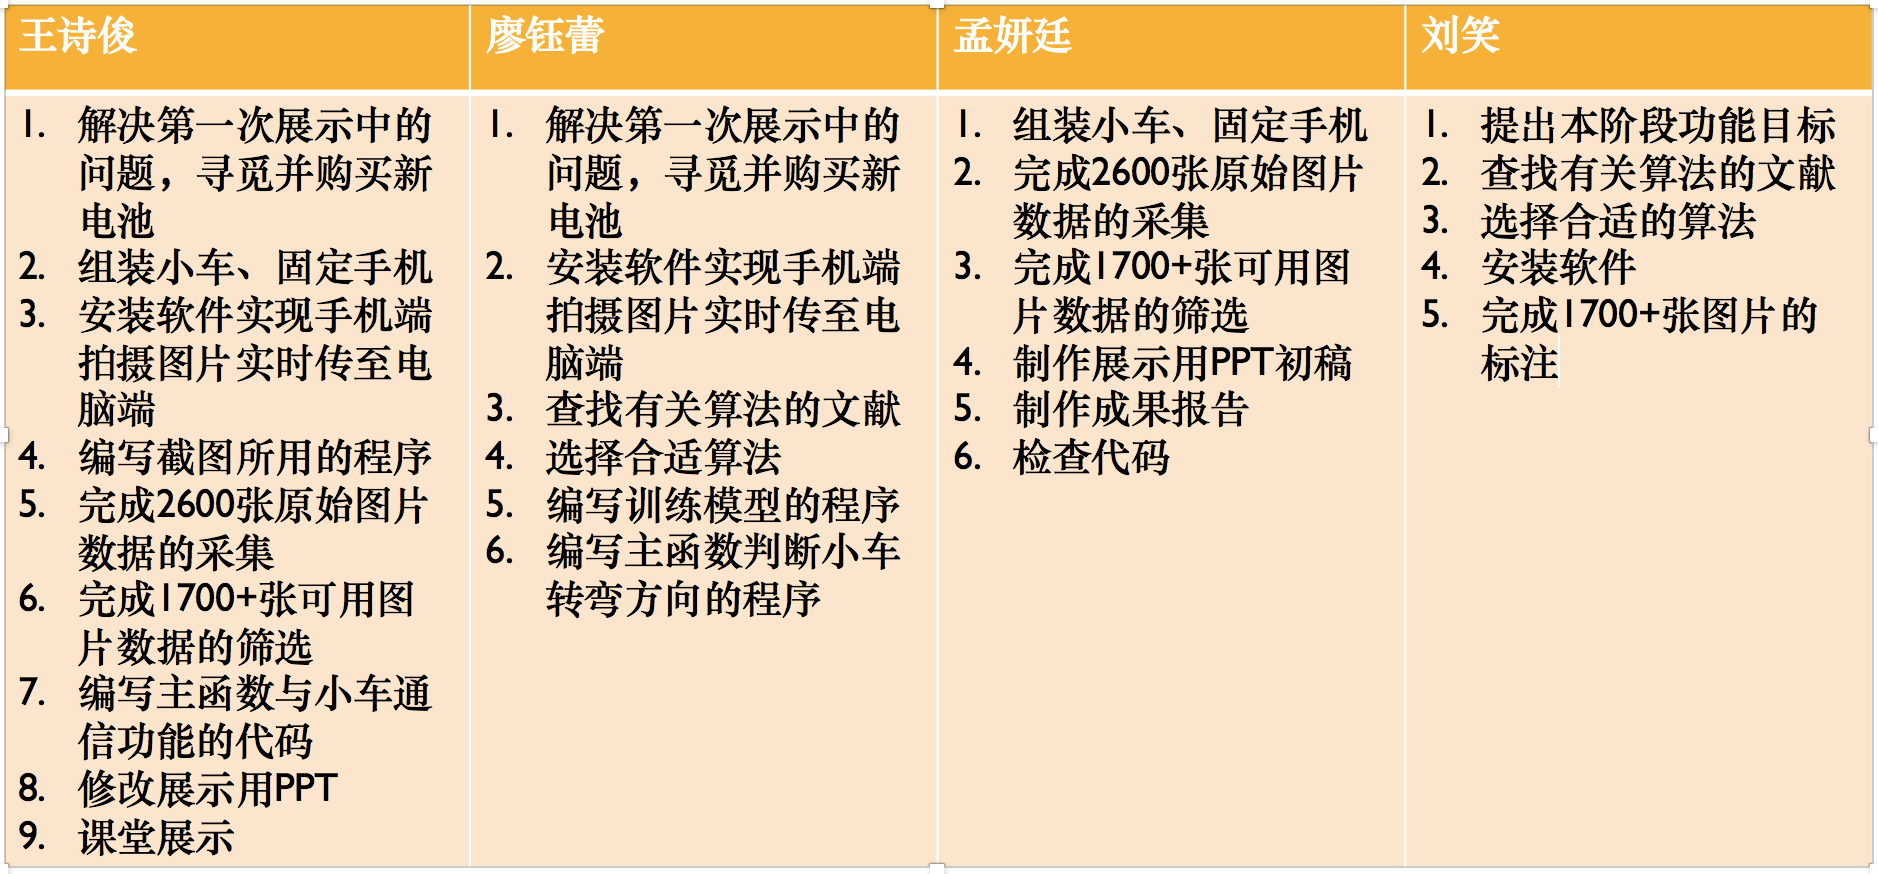
\includegraphics[scale=0.4]{0.png}
\end{figure}

\indent\textbf{八\quad 参考文献:}\\
\indent Canny参考:http://homepages.inf.ed.ac.uk/rbf/HIPR2/canny.html\\
\indent SIFT参考:https://www.cs.ubc.ca/~lowe/papers/ijcv04.pdf\\
\indent k-means参考:http://www.onmyphd.com/?p=k-means.clustering\&ckattempt=1\\
\end{document}
